\chapter{Zpracování dat}
Vytvořené zařízení inerciální jednotky poskytuje poměrně velké množství dat které je možné různě zpracovávat. Kromě samotných dat z dvou IMU také zaznamenává měřené hodnoty z elektronického kompasu a GNSS modulu. V průběhu vypracování práce se ukázalo, že zpracovat data tak, abychom dosáhli uspokojivých výsledků není vůbec jednoduché a zasloužilo by si samo o sobě rozsah další práce. V této kapitole budou popsány zejména dva postupy zpracování měření, a to výpočet trajektorie čistě z pohybových rovnic a fůze dat s GNSS. Později bylo také zjištěno, že navigace čistě z inerciálních dat nedosahuje uspokojivých výsledků a je zapotřebí korekce dat z GNSS, který ovšem má často ve vnitřních prostorech velmi špatné pokrytí.

Všechny níže popsané skripty byly vytvořené v prostředí MATLAB, jelikož je v něm manipulace s vektory a maticemi jednoduchá. Také můžeme využít již hotových modelů chování senzorů a implementovaných filtrů z Navigation Toolboxu, který je stále poměrně rozsáhle rozšiřován. V elektronické příloze jsou kromě skriptů dostupná i vzorová naměřená data, převedena do formátu csv, které je možné použít k experimentování. Obsahují například chůzi napříč budovou a místností, jízdu autem na venkovním prostranství a měření jednotky v klidu.

\section{Výpočet trajektorie pomocí pohybových rovnic} \label{noFiltProcessing}
Jedná se o základní způsob zpracování dat, který byl popsán v kapitole \ref{INSalg}, které lze nejlépe vystihnout obrázkem  \ref{StrapdownBlock}. Nejdříve je vypočteno z prvního vzorku zrychlení natočení celého zařízení vůči zemi, tedy směr tíhového vektoru. Z tohoto důvodu je potřeba, aby zařízení bylo při začátku měření nepohyblivé. Následně jsou data z gyroskopu integrována numerickou lichoběžníkovou metodou, abychom získali změnu orientace jednotky, ke kterému je přičten výchozí stav.

Z těchto úhlů natočení je vypočtena rotační matice, pomocí které otočíme měřená data zrychlení z body framu do earth framu. Z tohoto rotovaného zrychlení je následně odečten vektor tíhového zrychlení a pomocí dvou dalších numerických integrací otočeného zrychlení vypočteme odhad trajektorie.

Pro demonstraci tohoto postupu byla vytvořena vzorová data chůze ve tvaru obdélníku o rozměrech 3,5 a 4 m. Na začátku a konci těchto měření byla jednotka položena nehybně na stole.

\begin{figure}[h]
     \centering
     \begin{subfigure}[b]{0.49\textwidth}
         \centering
         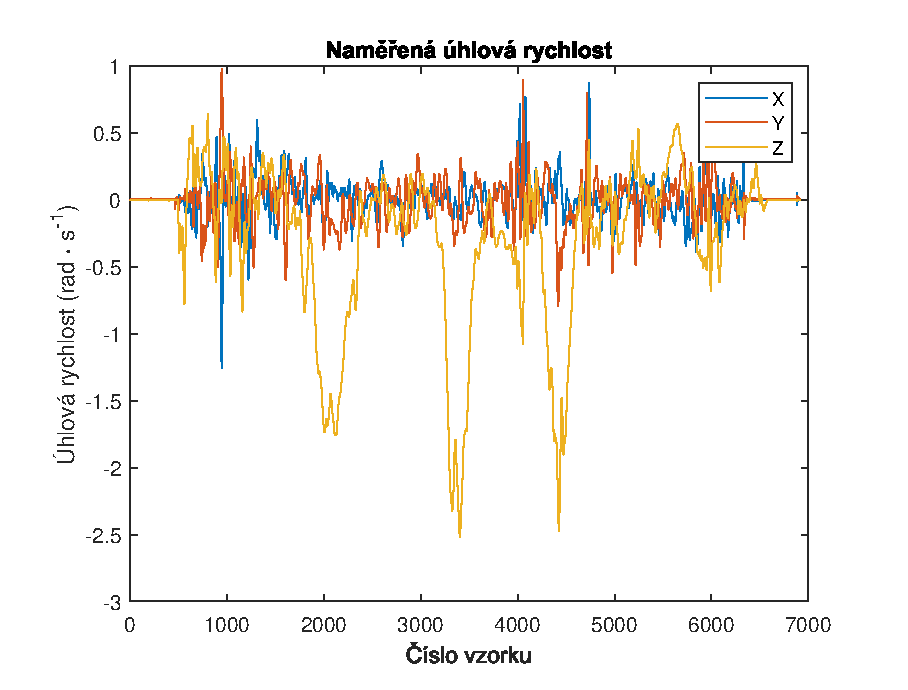
\includegraphics[width=\textwidth]{obrazky/matlab/1measAngularVel}
         \caption{Data z akcelerometru.}     
     \end{subfigure}
     \hfill
     \centering
     \begin{subfigure}[b]{0.49\textwidth}
         \centering
         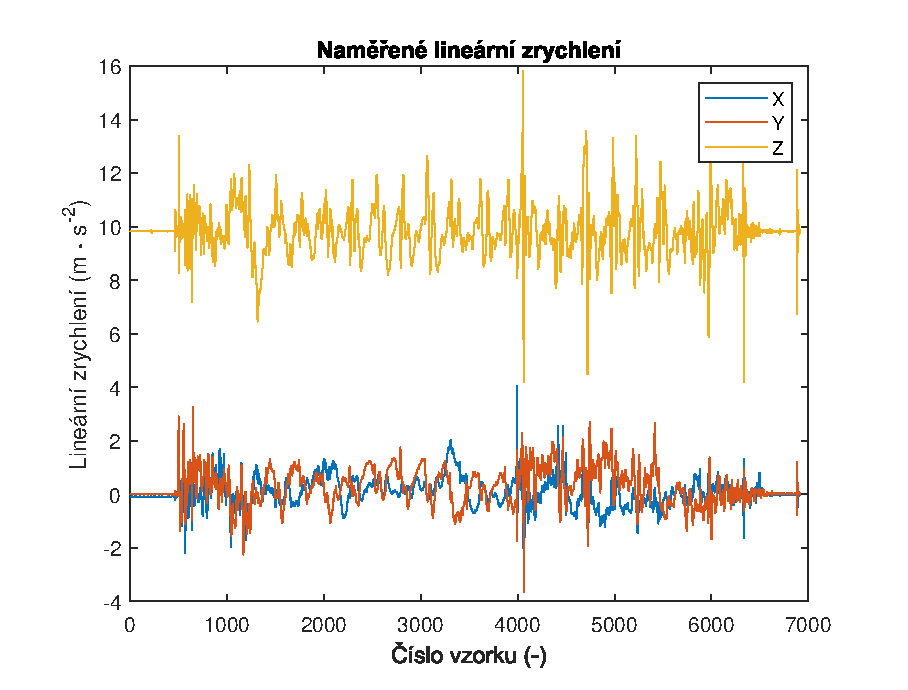
\includegraphics[width=\textwidth]{obrazky/matlab/1measAccel}
         \caption{Data z gyroskopu.}   
     \end{subfigure}

        \caption{Záznam dat IMU ADIS16505.}
        \label{fig:IMURawData}
\end{figure}

Na obrázku \ref{fig:IMURawData} jsou vidět nezpracovaná zaznamenaná data. Úhlová rychlost v ose Z obsahuje výrazné špičky, jedná se o otáčení v rozích pomyslného čtverce. Na datech akcelerometru je vidět, že celý čas měření byla jednotka převážně ve vodorovné pozici, jelikož lineární zrychlení v ose Z představuje tíhové zrychlení. Zákmity ve zrychlení jsou způsobeny kroky chůze.

\begin{figure}[h]
     \centering
     \begin{subfigure}[b]{0.49\textwidth}
         \centering
         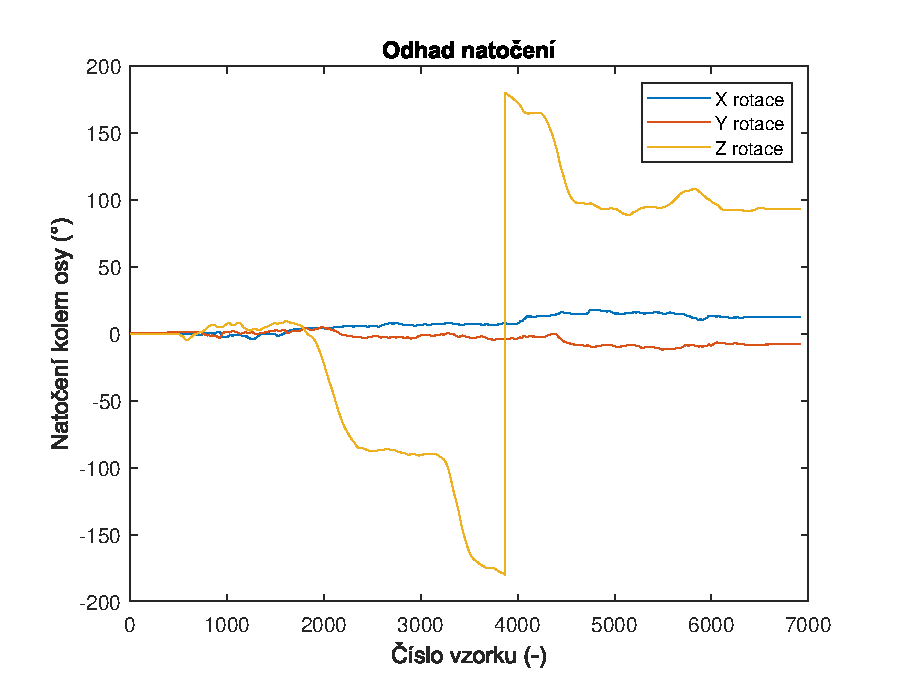
\includegraphics[width=\textwidth]{obrazky/matlab/1measOrient}
         \caption{Natočení jednotky.}   
         \label{fig:Rotation}  
     \end{subfigure}
     \hfill
     \centering
     \begin{subfigure}[b]{0.49\textwidth}
         \centering
         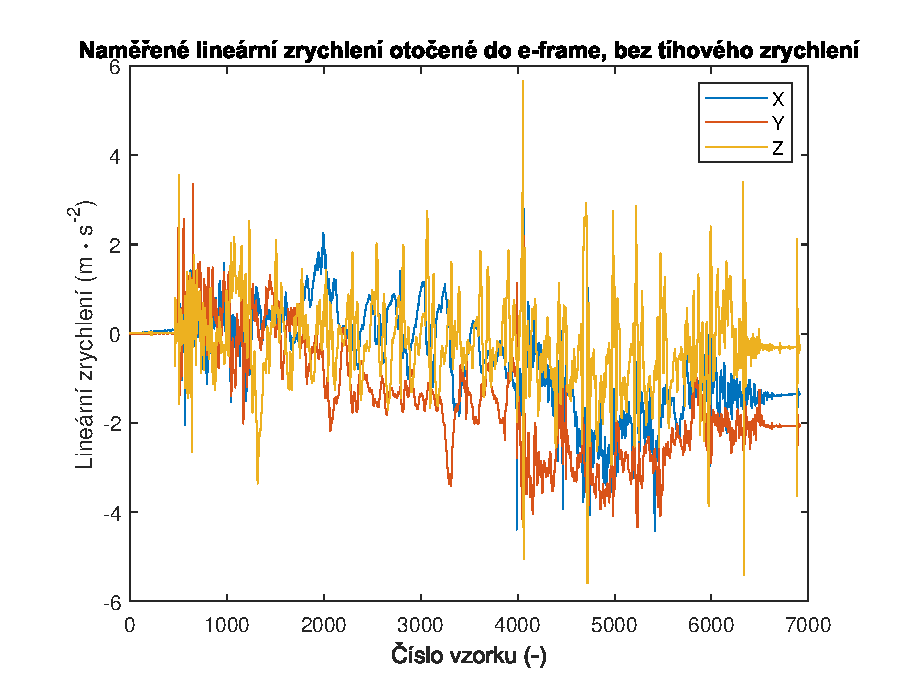
\includegraphics[width=\textwidth]{obrazky/matlab/1measAccelEframeWithoutG}
         \caption{Zrychlení v e-frame bez tíhového.}   
         \label{fig:AccelWithoutG}  
     \end{subfigure}

        \caption{Výsledky po první integraci.}
        \label{fig:rotationAccel}
\end{figure}

Po integraci dat úhlové rychlosti můžeme určit natočení jednotky (znázorněno na obrázku \ref{fig:Rotation} ) a rotovat vektory zrychlení do e-frame. Po odečtení tíhového zrychlení z osy Z dostaneme data na obrázku \ref{fig:AccelWithoutG}.

Na obou grafech z obrázku \ref{fig:rotationAccel} je patrně vidět problém čistě inerciální navigace, kde na konci měření není zrychlení, nebo natočení v osách X a Y nulové. To je způsobené kumulováním chyby při integraci dat. Toto bývá označováno jako gyro drift. Často jsou chyby potlačovány použitím kalmanova filtru, kde je drift gyroskopu kompenzován dlouhodobým měřením směru tíhového zrychlení, což je vhodné pro případ, že by naším cílem bylo určit pouze náklon v prostoru. Ovšem vzhledem k tomu, že použití filtrů přináší časovou prodlevu v ustálení měření orientace, tak jsou data akcelerometru stále krátkodobě natáčena ve špatném směru, což po následné integraci na rychlost a trajektorii stále přináší velkou chybu.

Po následných dvou numerických integrací zrychlení můžeme výslednou trajektorii reprezentovat v 3D prostoru obrázkem \ref{fig:Trajectory}, kde je v počátku mírně vidět tendence chůze v přímce, ale poté nastává integrací chyby úplné znehodnocení dat. 

\begin{figure}[h]
     \centering
         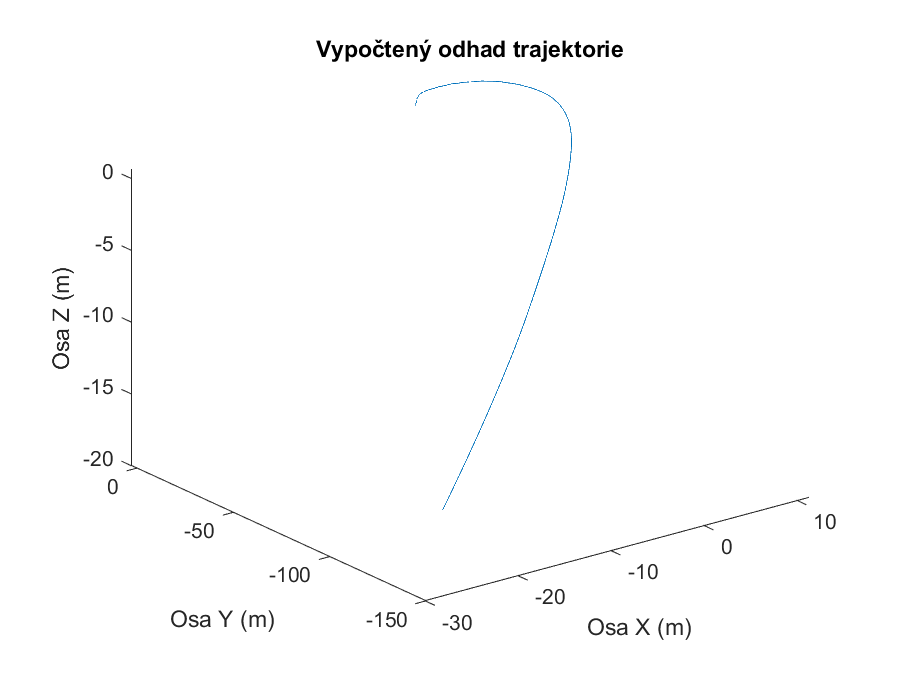
\includegraphics[width=0.5\textwidth]{obrazky/matlab/1measTraj}
         \caption{Odhad trajektorie.}
        \label{fig:Trajectory}
\end{figure}

\section{Vliv kalibrace senzorů}
Za krátkou zmínku stojí i porovnání vlivu kalibrace senzorů na výsledná data. Na to můžeme použít skript z kapitoly \ref{noFiltProcessing}. Přestože odhad trajektorie nemá moc velkou vypovídající hodnotu, tak přesnost senzorů můžeme alespoň částečně posoudit například tím, jak moc se změřené zrychlení v e-framu s odečteným tíhovým zrychlením na konci měření když je zařízení v klidu odchyluje od nuly. Byla provedena dvě obdobná měření při chůzi s jednotkou trajektorie stejného tvaru z předchozí kapitoly, bez kalibrace a s kalibrací.

\begin{figure}[h]
     \centering
     \begin{subfigure}[b]{0.49\textwidth}
         \centering
         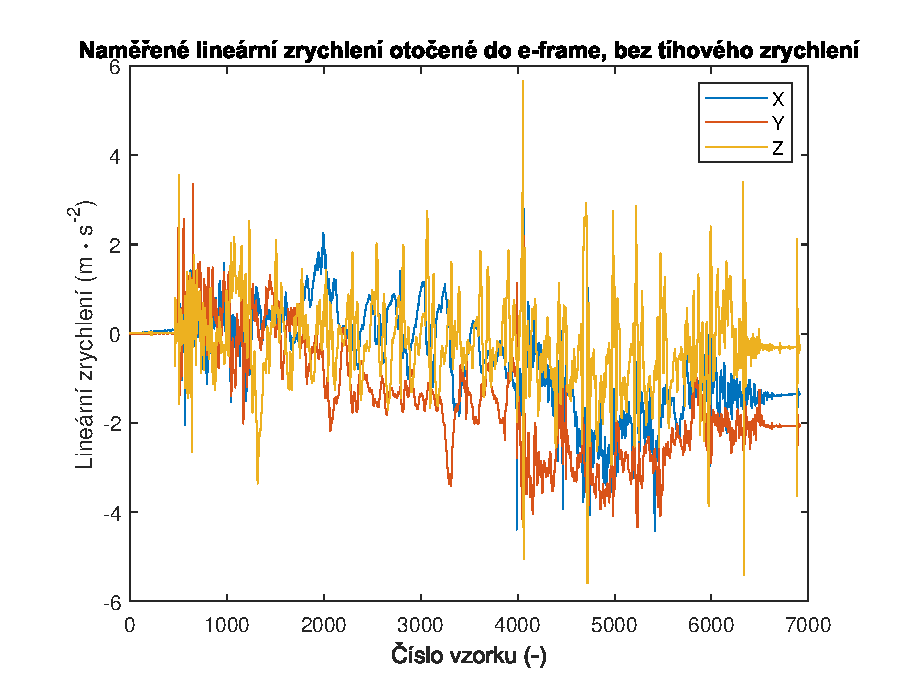
\includegraphics[width=\textwidth]{obrazky/matlab/1adisNoCal}
         \caption{ADIS16505 bez kalibrace.}   
         \label{fig:adisNoCal}  
     \end{subfigure}
     \hfill
     \centering
     \begin{subfigure}[b]{0.49\textwidth}
         \centering
         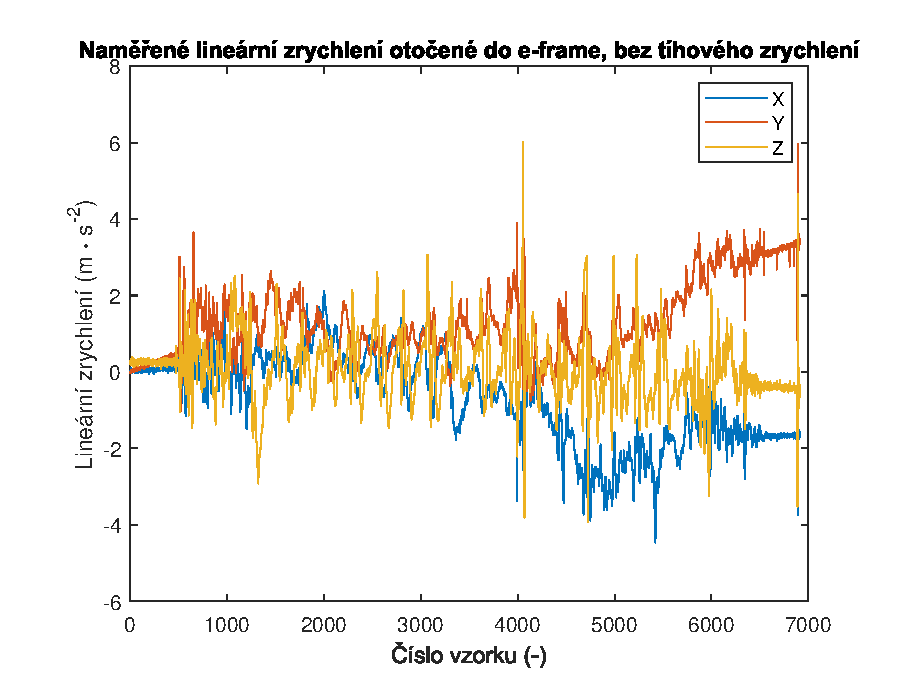
\includegraphics[width=\textwidth]{obrazky/matlab/1mpuNoCal}
         \caption{MPU6050 bez kalibrace.}   
         \label{fig:mpuNoCal}  
     \end{subfigure}
     
     
     \centering
     \begin{subfigure}[b]{0.49\textwidth}
         \centering
         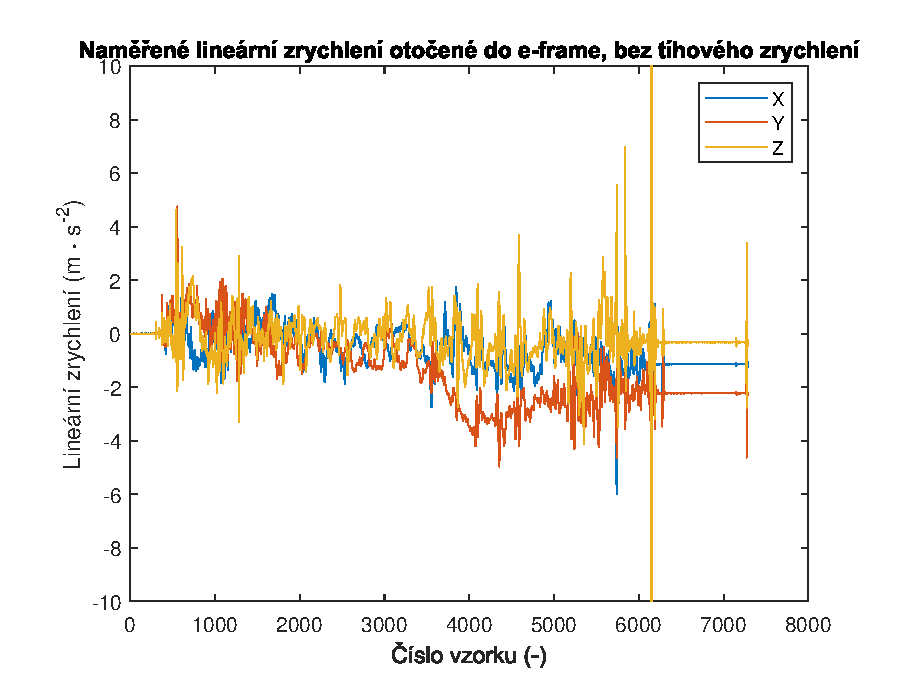
\includegraphics[width=\textwidth]{obrazky/matlab/1adisWithCal}
         \caption{ADIS16505 s kalibrací.}   
         \label{fig:AdisWithCal}  
     \end{subfigure}
     \hfill
     \centering
     \begin{subfigure}[b]{0.49\textwidth}
         \centering
         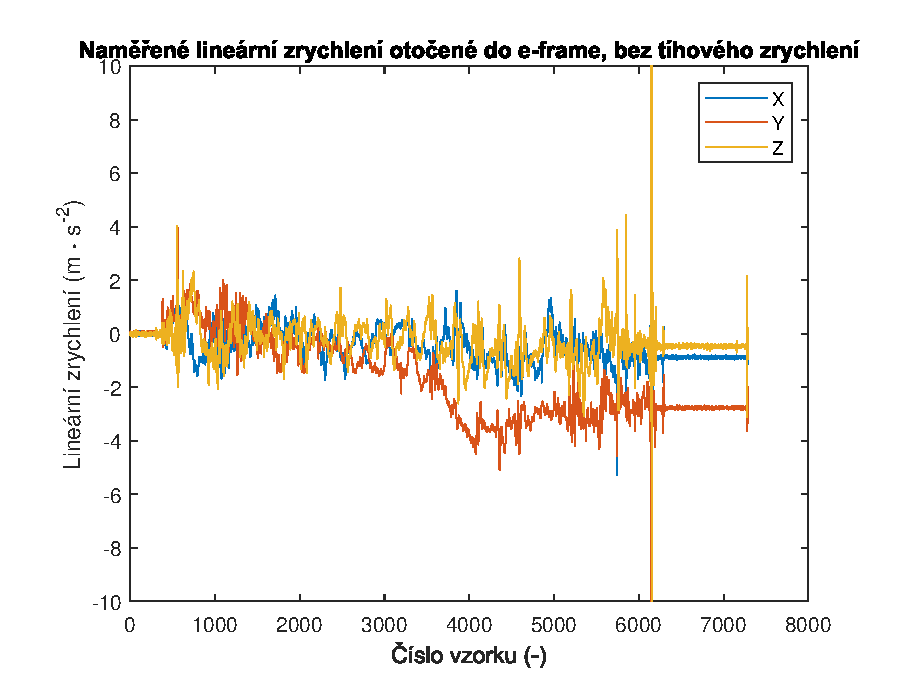
\includegraphics[width=\textwidth]{obrazky/matlab/1mpuWithCal}
         \caption{MPU6050 s kalibrací.}   
         \label{fig:mpuWithCal}  
     \end{subfigure}
        \caption{Porovnání senzorů s kalibrací a bez kalibrace.}
        \label{fig:calibrationComp}
\end{figure}

Na obrázku \ref{fig:calibrationComp} můžeme vidět porovnání dvou měření se zpracovanými daty z obou IMU. ADIS16505 dosahuje na konci měření maximální odchylku zrychlení zhruba $ \SI[per-mode = symbol]{2}{\metre\per\second\squared} $ s i bez kalibrace. To odpovídá tomu, že se jedná o poměrně přesný a nákladný senzor. Po kalibraci jsou totiž konstanty gainu pro všechny osy akcelerometru většinou řádově rovny 0,99990 a lepší, není jej potřeba tedy téměř kalibrovat. Situace je ovšem jiná u IMU MPU6050, které bez kalibrace dosahuje dvojnásobné odchylky od ADIS16505, zatímco po kalibraci je jeho odchylka zhruba srovnatelná s přesnějším senzorem.

Z tohoto můžeme usoudit, že i takto poměrně jednoduchá metoda kalibrace má poměrně dost pozitivní dopady na výsledky měření levnějších IMU.

\section{Fůze dat s GNSS}
Na fúzi inerciálních dat byl použit filtr s připravenými modely senzorů akcelerometru, gyroskopu, magnetometru a GNSS. Na odhad polohy využívá rozšířený kalmanův filtr s 22 prvkovým stavovým vektorem, který kromě pozice sleduje i natočení, rychlost biasy akcelerometru, gyroskopu a magnetometru a odhad magnetického pole Země. \cite{M7nvHLyk8N0V3ub2}

Pro zpracování dat byl použit vzorek měření jízdy autem ve venkovním prostředí, kde je  příjem GNSS signálu spolehlivější. Na obrázku \ref{fig:gnssOriginal} jsou zobrazena naměřená data polohy GNSS přijímače, na obrázku \ref{fig:gnnsIMUFusion} je zobrazen odhad polohy z fúze GNSS a IMU dat pomocí filtru \texttt{insFilterMARG}. Jak je vidět, tak výsledky nejsou optimální, zejména ve výchozí pozici měření, kde dochází k ustálení filtru.

Přesnost výsledků filtru je poměrně závislá na správném nastavení kovarianční matice 22 prvkového stavového vektoru a nastavení rozptylu šumu a biasu jednotlivých senzorů. Zde byly použity pouze odhady a výchozí hodnoty těchto veličin. Pro správné fungování bude pravděpodobně potřeba tyto hodnoty přesně vyčíslit, což umožňují například některé ladicí funkce Navigation toolboxu, ty ovšem využívají buď modelů konkrétních použitých součástek, nebo na měření se zařízením, se kterým bylo pohybováno po přesně definované trajektorii, což vzhledem k časové náročnosti takového měření a předchozích částí této práce nebylo realizováno.  

\begin{figure}[h]
     \centering
         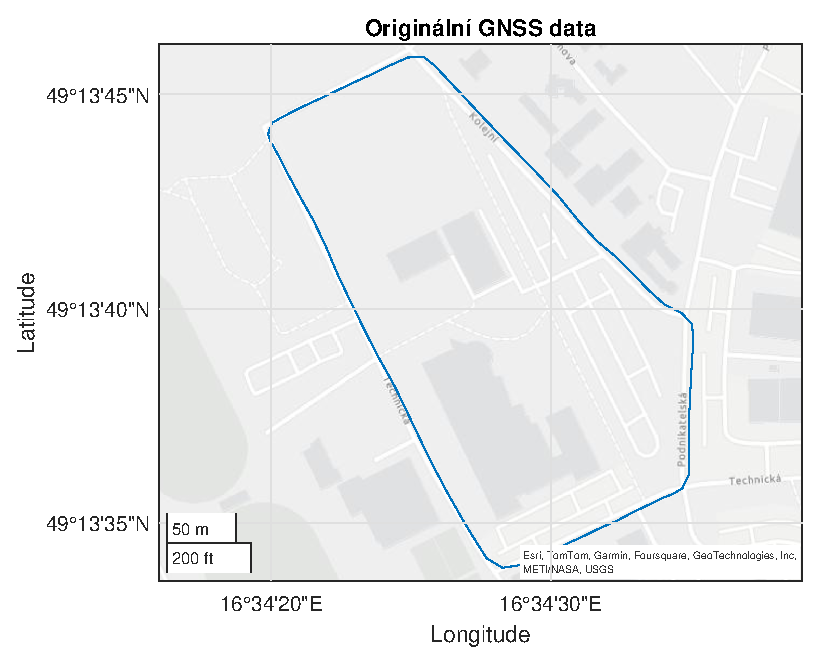
\includegraphics[width=0.5\textwidth]{obrazky/matlab/2gnss}
         \caption{Naměřená GNSS data.}
        \label{fig:gnssOriginal}
\end{figure}

\begin{figure}[h]
     \centering
     \begin{subfigure}[b]{0.49\textwidth}
         \centering
         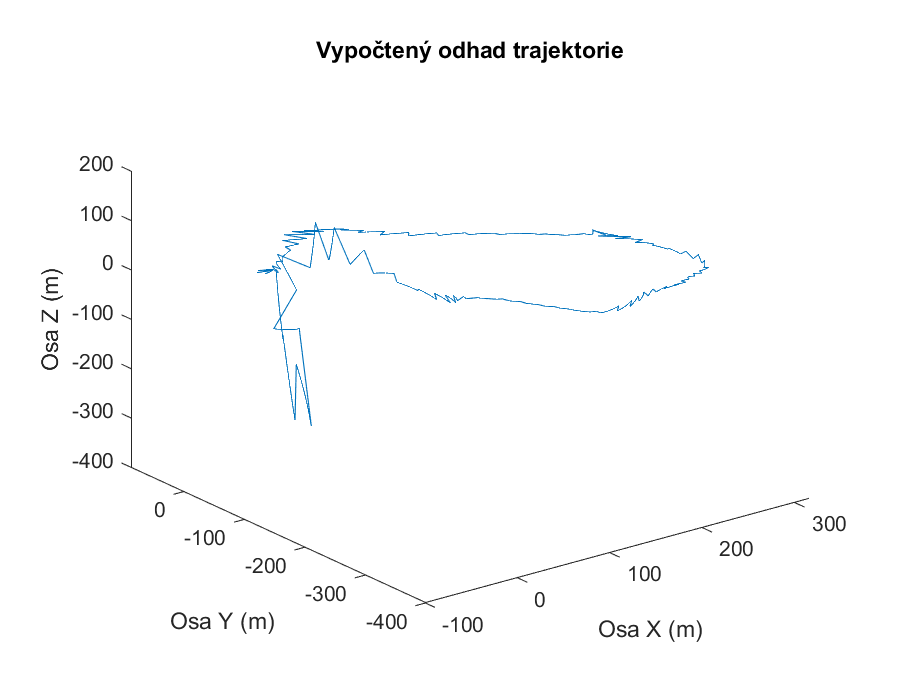
\includegraphics[width=\textwidth]{obrazky/matlab/2gnssIMU3d}
         \caption{Odhad trajektorie v 3D prostoru.}   
         
     \end{subfigure}
     \hfill
     \centering
     \begin{subfigure}[b]{0.49\textwidth}
         \centering
         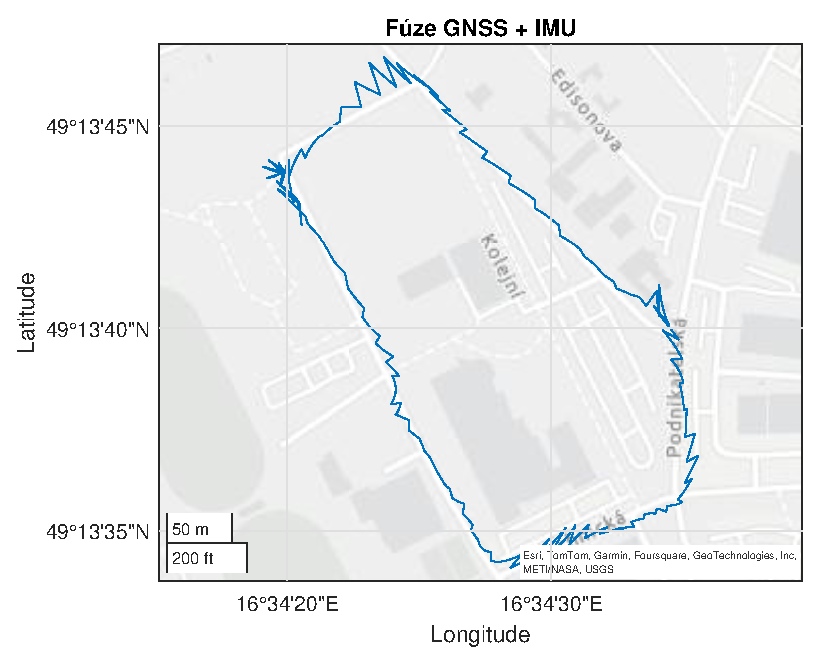
\includegraphics[width=\textwidth]{obrazky/matlab/2gnssIMU}
         \caption{Odhad trajektorie na mapě.}   
         
     \end{subfigure}
     
     \caption{Odhad trajektorie z fúze dat GNSS a IMU.}
     \label{fig:gnnsIMUFusion}  
\end{figure}

\chapter{Koncepce laboratorní úlohy}
Vzhledem k poměrně velké univerzálnosti vytvořeného hardwaru a obslužných skriptů jsou možnosti využití tohoto zařízení poměrně velké. Jako koncepci laboratorní úlohy můžeme zmínit třeba dvě následující.
\section{Analýza využití GNSS, dostupnost signálu a obsluha}
Tato laboratorní úloha by se mohla týkat analýzy dostupnosti a využití GNSS signálů uvnitř a vně budov, obsluhy a fungování navigačních modulů. 

Základní informace o stavu GNSS modulu v zařízení je možné zobrazovat na displeji jednotky. Také díky tomu, že je zapojený USB port GNSS modulu NEO-M8U do interního rozbočovače zařízení, lze využít například jakýkoliv terminál sériového rozhraní, nebo obslužnou aplikaci u-center od výrobce Ublox pro zobrazení dostupných satelitů navigačních systémů a jejich síly signálu, zaznamenat časovou závislost počtu satelitů od doby zapnutí zařízení, nebo faktory ovlivňující kvalitu GNSS signálu (překážky, atmosferické podmínky\ldots). Použitý GNSS modul podporuje všechny světové navigační systémy, lze tedy zaznamenat i počet dostupných satelitů jednotlivých systémů (GPS, BeiDou, Glonass, Galileo). Laboratorní úloha se také může věnovat dekódování NMEA zpráv, nebo určení přesnosti změřené polohy.

\begin{figure}[h]
     \centering
         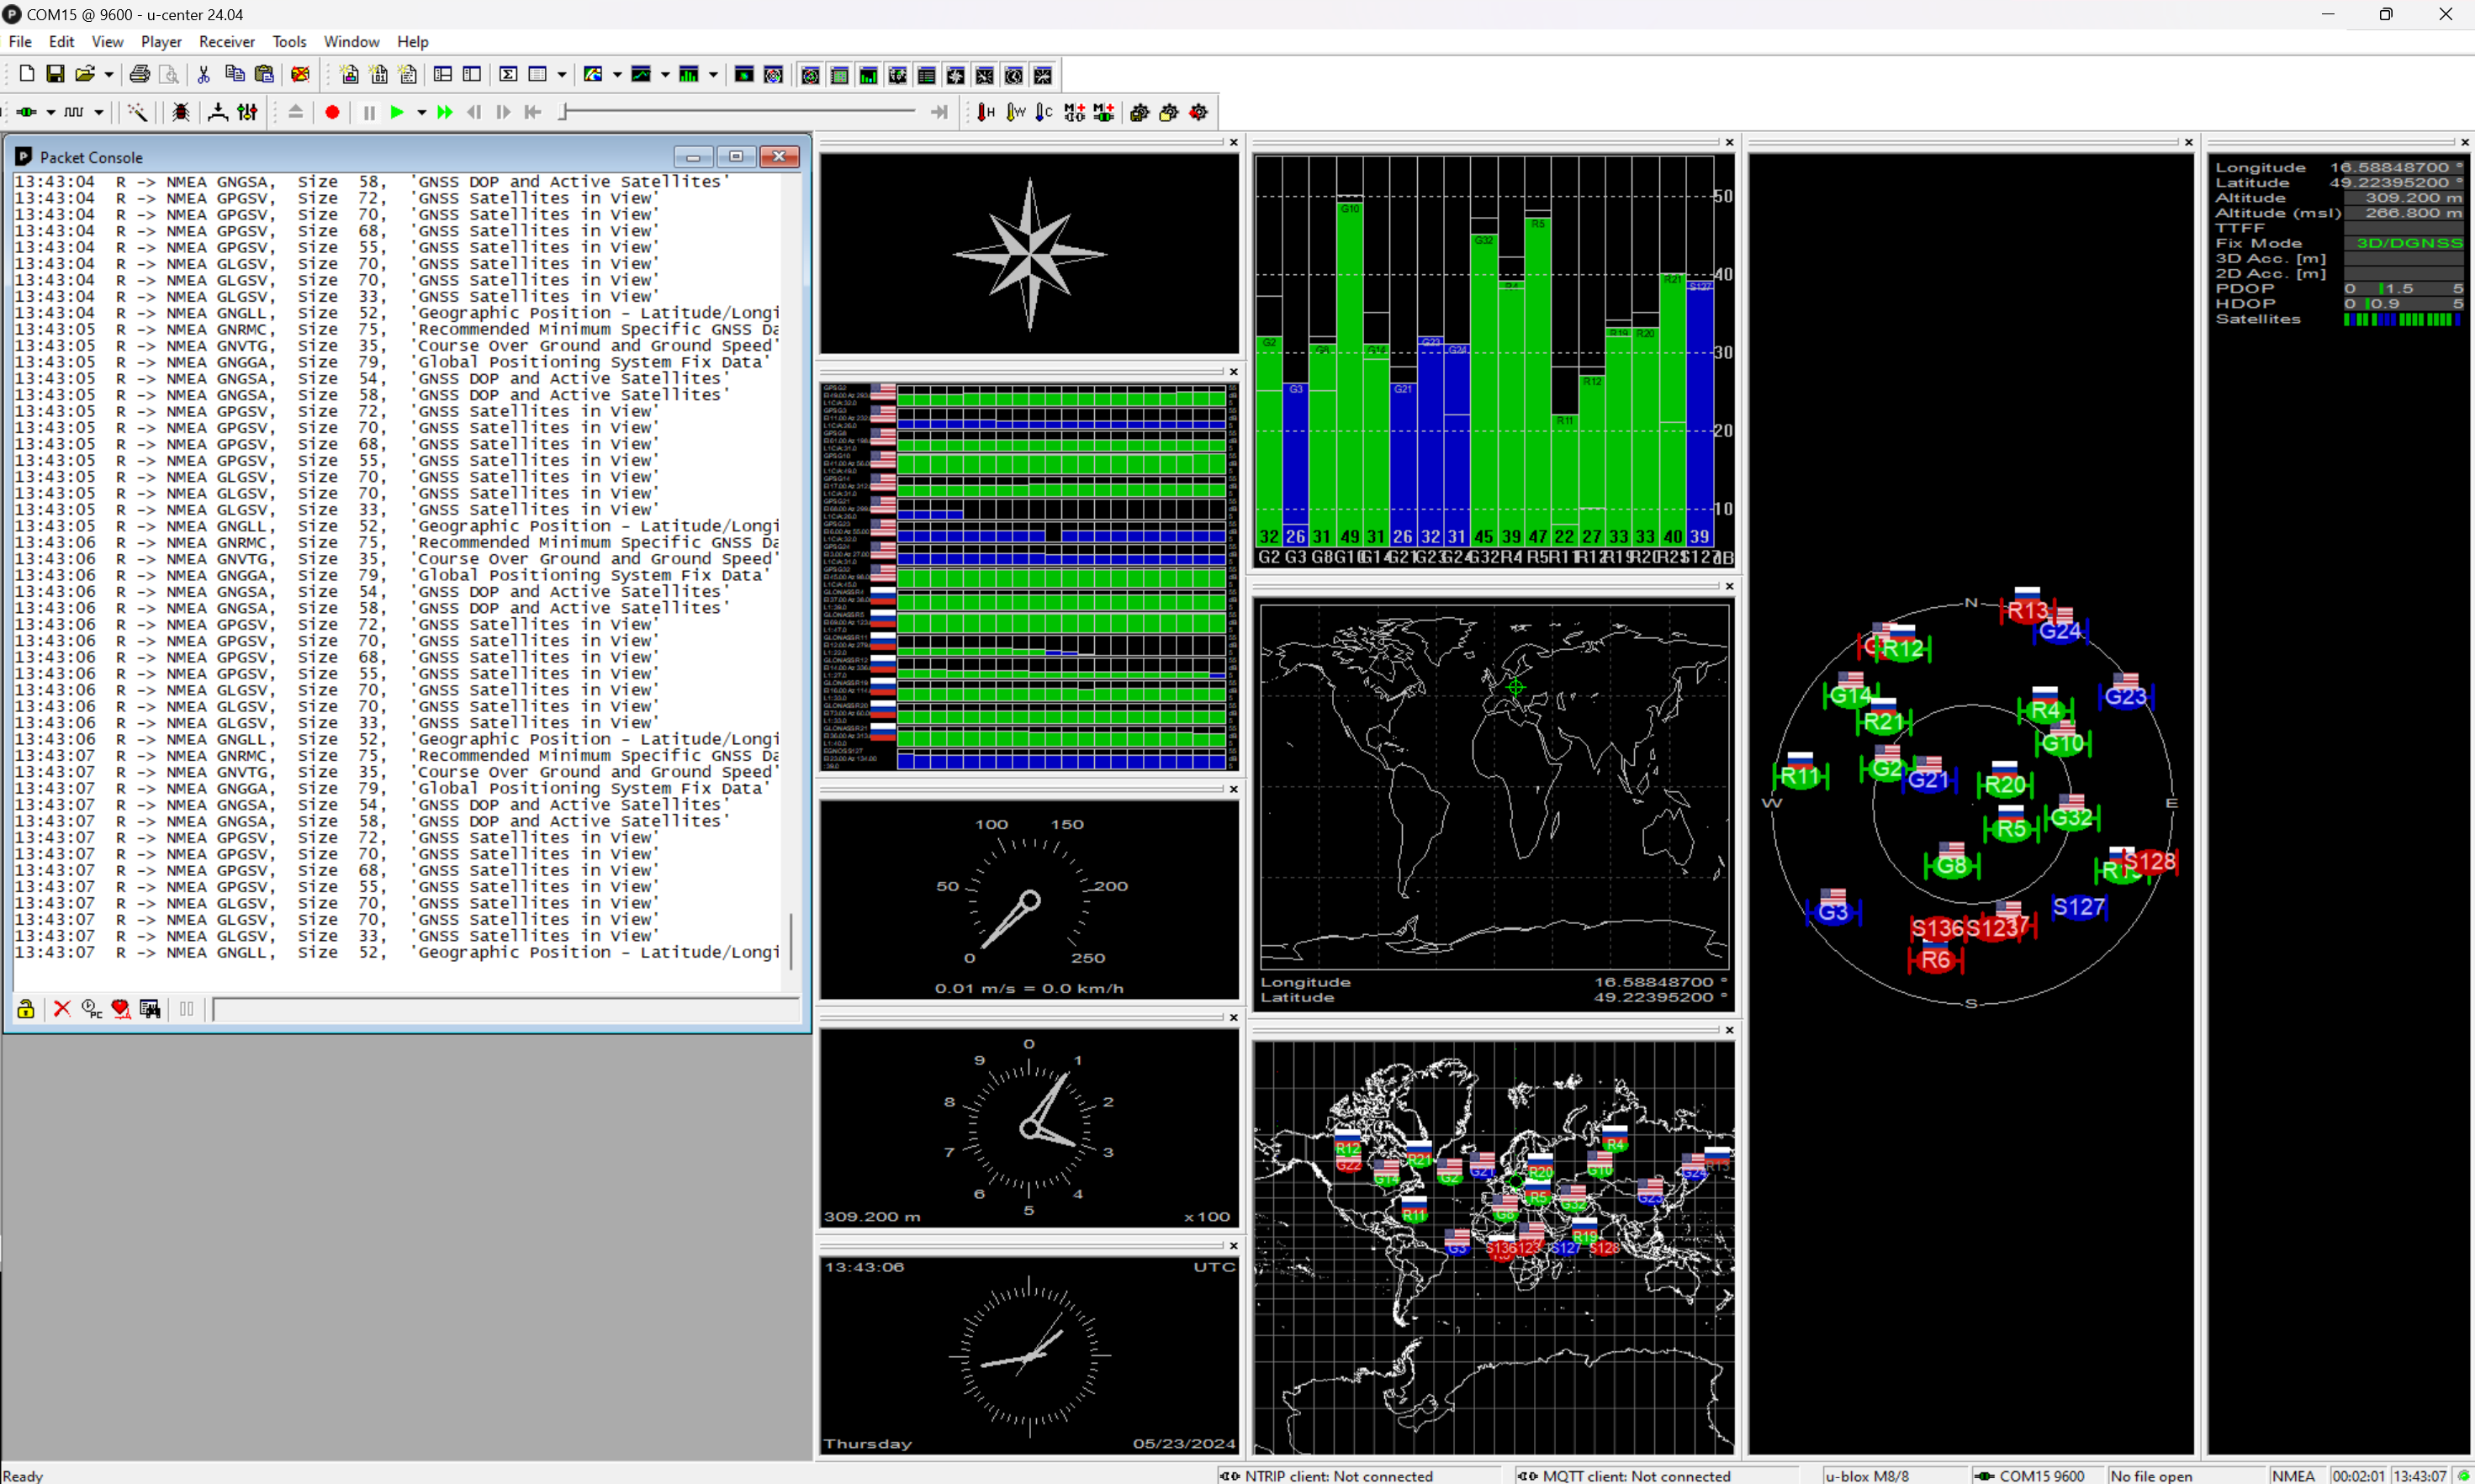
\includegraphics[width=0.99\textwidth]{obrazky/uCenter}
         \caption{Obslužná aplikace u-center.}
        \label{fig:uCenter}
\end{figure}

\section{Princip fungování IMU, vliv kalibrace a určení náklonu a polohy inerciální jednotkou}
Tato laboratorní úloha může být zaměřena na popsání principu fungování IMU, jaké veličiny lze měřit pomocí inerciálních senzorů, vliv a způsob kalibrace, zobrazení naměřených dat a jednotlivých dílčích veličin (zrychlení, orientace, rychlost, úhel), faktory ovlivňující nepřesnost výsledku a fúze dat s ostatními senzory. 

Pomocí zobrazených veličin na displeji lze zobrazit všechny měřené údaje zařízením. Lze jednoduše znázornit měření tíhového pole akcelerometrem v případě, že je jednotka v klidu. Následně lze pohybem se zařízením reprezentovat změny úhlové rychlosti a zrychlení. Také je možné výpočtem velikosti vektoru tíhového zrychlení otestovat přesnost senzorů před a po kalibraci, popřípadě i kalibrační konstanty vypočítat ručně pomocí dodaného kalibračního skriptu v MATLABu. Dále je možné reprezentovat z naměřených dat jednotlivé veličiny po integraci z čistě inerciální navigace a problémy spjaté s její nepřesností. Také můžeme využít skriptu na fúzi dat a otestovat její fungování, na to by bylo ovšem vhodné ještě zpracování dat vylepšit, abychom dosáhli uspokojivých výsledků.

